\chapter{Ferramentas de desenvolvimento}
\label{Ferramentasdedesenvolvimento}

\begin{chapquote}{Autor desconhecido}
``Existem duas maneiras de escrever programas sem erros; somente a terceira funciona.''
\end{chapquote}

Em geral, o conjunto de ferramentas de programação usadas para criar um programa é chamado de ferramentas de desenvolvimento. Para os fins deste texto, a cadeia de ferramentas consiste no seguinte:
\begin{itemize}
	\item Assembler (montador)
	\item Linker (ligador)
	\item Loader (carregador)
	\item Debugger (depurador)
\end{itemize}

Embora existam muitas opções para a cadeia de ferramentas, este texto usa um conjunto bastante padrão de ferramentas de código aberto que funcionam bem juntas e oferecem suporte total ao ambiente x86 de 64 bits.

Cada uma dessas ferramentas de programação é explicada nas seções a seguir.
\section{Visão geral de montagem/link/carga}
Em termos gerais, o processo de montar, \textit{linkar} e carregar é como os arquivos de origem escritos pelo programador são convertidos em um programa executável.

O arquivo de origem legível por humanos é convertido em um arquivo-objeto pelo assembler. Na forma mais básica, o arquivo-objeto é convertido em um arquivo executável pelo linker. O carregador carregará o arquivo executável na memória.

Uma visão geral do processo é fornecida no diagrama a seguir.

\tikzstyle{decision} = [diamond, draw, fill=blue!20, 
text width=4.5em, text badly centered, node distance=3cm, inner sep=0pt]
\tikzstyle{block} = [rectangle, draw, fill=blue!20, 
text width=5em, text centered, rounded corners, minimum height=4em]
\tikzstyle{bin} = [rectangle, draw, fill=blue!40, 
text width=5em, text centered, minimum height=4em]
\tikzstyle{line} = [draw, -latex']
\tikzstyle{cloud} = [draw, ellipse,fill=red!20, node distance=3cm,
minimum height=2em]

\tikzstyle{doc}=[%
draw,
thick,
align=center,
color=black,
shape=document,
minimum width=20mm,
shape=document,
inner sep=2ex,
]

\begin{tikzpicture}[node distance = 2.5cm, auto]
% Place nodes
\node [block] (init) {Assembler};
\node[doc] at ([shift=(0:-3cm)]init) (assembly) {Fonte em\\ linguagem\\ assembly};
\node [bin, below of=init] (objeto) {Arquivo objeto};
\node [block, below of=objeto] (link) {Link};
\node [doc, left of=objeto, node distance=3cm] (listagem) {Arquivo\\listagem};
\node [bin, node distance=3cm] at ([shift=(5:2.5cm)]objeto) (outro) {Outro arquivo objeto (se houver)};
\node [bin, node distance=3cm] at ([shift=(-4:3cm)]outro) (biblio) {Rotinas da biblioteca (se houver)};
\node [bin, below of=link] (exe) {Executável};
\node [bin, left of=exe] (shared) {Arquivos de objetos compartilhados};
\node [block, right of=exe, node distance=3cm] (load) {Load};
\node [block, below of=exe, node distance=3cm] (ram) {RAM};
% Draw edges
\path [line] (assembly) -- (init);
\path [line] (init) -- (objeto);
\path [line] (init) -- (listagem);
\path [line] (objeto) -- (link);
\path [line, dashed] (outro) -- (link);
\path [line, dashed] (biblio) |- (link);

\path [line] (link) -- (exe);
\path [line] (exe) -- (load);
\path [line] (load) -- (ram);
\path [line, dashed] (shared) -- (ram);


\end{tikzpicture}

As etapas de montagem, ligação e carregamento são descritas com mais detalhes nas seções a seguir.

\section{Assembler (montador)}
O assembler é um programa que lê um arquivo de entrada em linguagem \textit{assembly} e converte o código em um arquivo binário de linguagem de máquina. O arquivo de entrada é um arquivo fonte em linguagem \textit{assembly} que contém instruções em linguagem \textit{assembly} em formato legível por humanos. A saída da linguagem de máquina é conhecida como um arquivo de objeto. Como parte desse processo, os comentários são removidos e os nomes das variáveis e rótulos são convertidos em endereços apropriados (conforme exigido pela CPU durante a execução).

O assembler usado neste texto é o \textbf{yasm} 25. Links para o site e documentação do \textbf{yasm} podem ser encontrados no Capítulo \ref{cap1}, Introdução.

\subsection{Comandos de montagem}
O comando do \textbf{yasm} apropriado para ler o arquivo de origem da linguagem \textit{assembly}, como o exemplo do capítulo anterior, é o seguinte:
\begin{center}
	\textbf{yasm -g dwarf2 -f elf64 exemplo.asm -l exemplo.lst}
\end{center}

Observe que o \textit{-l} é uma letra \textbf{L} minúscula com traço na frente (que pode ser facilmente confundida com o número $ 1$).

A opção \textbf{-g dwarf2} é usada para informar ao montador para incluir informações de depuração no arquivo de objeto final. Isso aumenta o tamanho do arquivo de objeto, mas é necessário para permitir uma depuração eficaz. O \textbf{-f elf64} informa o montador para criar o arquivo objeto no formato \textbf{ELF64}, que é apropriado para sistemas baseados em \textit{Linux de 64 bits}. O \textbf{exemplo.asm} é o nome do arquivo de origem da linguagem \textit{assembly} para entrada. O \textbf{-l exemplo.lst} (traço minúsculo, letra L) informa ao montador para criar um arquivo de lista denominado \textit{exemplo.lst}.

Se ocorrer um erro durante o processo de montagem, ele deve ser resolvido antes de prosseguir para a etapa de link.

\subsection{Arquivo de listagem}
Além disso, o montador é opcionalmente capaz de criar um arquivo de listagem. O arquivo de listagem mostra o número da linha, o endereço relativo, a versão em linguagem de máquina da instrução (incluindo referências de variáveis) e a linha de origem original. O arquivo de listagem pode ser útil durante a depuração.

Por exemplo, um fragmento da seção de dados do arquivo de lista, do programa de exemplo no capítulo anterior, é o seguinte:

\begin{verbatim}
36 00000009 40660301	dVar1	  dd	17000000
37 0000000D 40548900	dVar2	  dd	9000000
38 00000011 00000000	dResult	dd	0
\end{verbatim}

Na primeira linha, \textbf{36} é o número da linha. O próximo número, \textbf{0x00000009}, é o endereço relativo na área de dados de onde a variável será armazenada. Como \textbf{dVar1} é uma palavra dupla, que requer quatro bytes, o endereço da próxima variável é \textbf{0x0000000D}. A variável \textbf{dVar1} usa \textbf{4} bytes como endereços \textbf{0x00000009}, \textbf{0x0000000A}, \textbf{0x0000000B} e \textbf{0x0000000C}. O resto da linha é a declaração de dados conforme digitada no arquivo-fonte original da linguagem \textit{assembly}.

O \textbf{0x40660301} é o valor, em hexadecimal, conforme colocado na memória. O \textbf{$ 17000000_{10} $}  é \textbf{0x01036640}. Lembrando que a arquitetura é \textit{little-endian}, o byte menos significativo (\textbf{0x40}) é colocado no endereço de memória mais baixo. Como tal, o \textbf{0x40} é colocado no endereço relativo \textbf{0x00000009}, o próximo byte, \textbf{0x66}, é colocado no endereço \textbf{0x0000000A} e assim por diante. Isso pode ser confuso, pois à primeira vista o número pode aparecer invertido ou truncado (dependendo de como é visualizado).

Para ajudar a visualizar, a imagem da memória seria a a da Figura \ref{fig:litllelayout}:

\tikzstyle{memoria} = [rectangle, draw, fill=blue!20, 
text width=4em, text centered]

\begin{figure}[h]
\begin{center}
		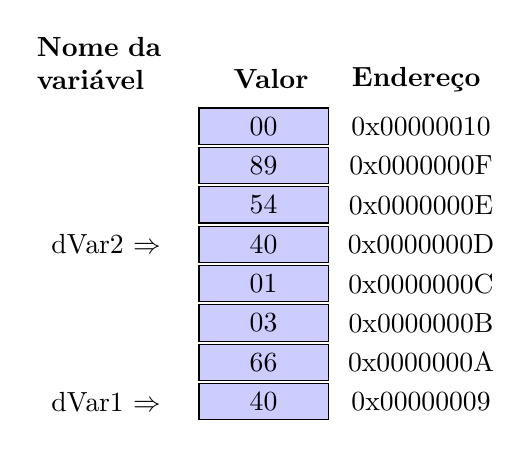
\begin{tikzpicture}
\node [text width=5em,xshift=0.5cm,] (nome) {\textbf{Nome da variável}};
\node [text width=5em, xshift=3cm, yshift=-0.2cm] (valor)  {\textbf{Valor}};
\node [text width=5em, xshift=4.5cm, yshift=-0.2cm] (endereco) {\textbf{Endereço}};
\node [memoria, xshift=2.5cm, yshift=-0.8cm ]  {00};
\node [xshift=4.5cm, yshift=-0.8cm ]  {0x00000010};
\node [memoria, xshift=2.5cm, yshift=-1.3cm ]  {89};
\node [xshift=4.5cm, yshift=-1.3cm ]  {0x0000000F};
\node [memoria, xshift=2.5cm, yshift=-1.8cm ]  {54};
\node [xshift=4.5cm, yshift=-1.8cm ]  {0x0000000E};
\node [memoria, xshift=2.5cm, yshift=-2.3cm ]  {40};
\node [xshift=0.5cm, yshift=-2.3cm ]  {dVar2 $\Rightarrow$};
\node [xshift=4.5cm, yshift=-2.3cm ]  {0x0000000D};
\node [memoria, xshift=2.5cm, yshift=-2.8cm ]  {01};
\node [xshift=4.5cm, yshift=-2.8cm ]  {0x0000000C};
\node [memoria, xshift=2.5cm, yshift=-3.3cm ]  {03};
\node [xshift=4.5cm, yshift=-3.3cm ]  {0x0000000B};
\node [memoria, xshift=2.5cm, yshift=-3.8cm ]  {66};
\node [xshift=4.5cm, yshift=-3.8cm ]  {0x0000000A};
\node [memoria, xshift=2.5cm, yshift=-4.3cm ]  {40};
\node [xshift=4.5cm, yshift=-4.3cm ]  {0x00000009};
\node [xshift=0.5cm, yshift=-4.3cm ]  {dVar1 $\Rightarrow$};

\end{tikzpicture}
\end{center}
	\caption{Little-Endian, Layout de dados de múltiplas variáveis}
	\label{fig:litllelayout}
\end{figure}

Por exemplo, um fragmento da seção de texto do arquivo de lista, extraído do programa de exemplo no capítulo anterior, é o seguinte:

\begin{verbatim}
95                         last:
96 0000005A 48C7C03C000000	  mov		rax, SYS_exit
97 00000061 48C7C300000000	  mov		rdi, EXIT_SUCCESS	
98 00000068 0F05			            syscall
\end{verbatim}

Novamente, os números à esquerda são os números das linhas. O próximo número, \textbf{0x0000005A}, é o endereço relativo de onde a linha de código será colocada.

O próximo número, \textbf{0x48C7C03C000000}, é a versão em linguagem de máquina da instrução, em hexadecimal, que a CPU lê e entende. O resto da linha é a instrução de origem da linguagem \textit{assembly} original.

O rótulo, \textbf{last:}, não tem uma instrução em linguagem de máquina, pois o rótulo é usado para fazer referência a um endereço específico e não é uma instrução executável.

\subsection{Montador de dois passos}
O montador lerá o arquivo fonte e converterá cada instrução da linguagem \textit{assembly}, digitada pelo programador, em um conjunto de uns e zeros que a CPU sabe que é essa instrução. Os 1s e 0s são chamados de \textbf{linguagem de máquina}. Há uma correspondência de um para um entre as instruções em linguagem \textit{assembly} e a \textbf{linguagem de máquina binária}. Esse relacionamento significa que a linguagem de máquina, na forma de um arquivo executável, pode ser convertida novamente em linguagem \textit{assembly} legível por humanos. Claro, os comentários, nomes de variáveis e nomes de rótulos estão faltando, então o código resultante pode ser muito difícil de ler.

Conforme o montador lê cada linha da linguagem \textit{assembly}, ele gera um código de máquina para essa instrução. Isso funcionará bem para instruções que não realizam saltos. No entanto, para instruções que podem alterar o fluxo de controle (por exemplo, instruções \textbf{IF}, saltos incondicionais), o montador não é capaz de converter a instrução. Por exemplo, dado o seguinte fragmento de código:

\begin{verbatim}
       mov rax, 0
       jmp skipRest
       ...
       ...
    skipRest:
\end{verbatim}

Isso é conhecido como uma \textbf{referência antecipada}. Se o montador lê o arquivo de montagem uma linha por vez, ele não leu a linha onde \textbf{skipRest} está definido. Na verdade, ele nem sabe ao certo se \textbf{skipRest} está definido.

Esta situação pode ser resolvida lendo o arquivo de origem do \textit{assembly} duas vezes. Todo o processo é conhecido como \textbf{assembler} de duas passagens. As etapas necessárias para cada passagem são detalhadas nas seções a seguir.

\subsubsection{Primeiro passo}
As etapas realizadas na primeira passagem variam com base no projeto do montador específico. No entanto, algumas das operações básicas realizadas na primeira passagem incluem o seguinte:

\begin{itemize}
	\item Criar tabela de símbolos
	\item Expandir macros
	\item Avaliar expressões constantes
\end{itemize}

Uma macro é um elemento de programa que é expandido em um conjunto de instruções predefinidas pelo programador. Para obter mais informações, consulte o Capítulo \ref{cap:Macros}, Macros.

Uma expressão constante é uma expressão composta inteiramente de constantes. Como a expressão é apenas constante, ela pode ser totalmente avaliada no momento da montagem. Por exemplo, supondo que a constante \textbf{BUFF} seja definida, a seguinte instrução contém uma expressão constante;
\begin{verbatim}
mov rax, BUFF+5
\end{verbatim}

Este tipo de expressão constante é comumente usado em programas grandes ou complexos.

Os endereços são atribuídos a todas as instruções do programa. A tabela de símbolos é uma lista ou tabela de todos os símbolos de programa, nomes de variáveis e rótulos de programa e seus respectivos endereços no programa.

Conforme apropriado, algumas diretivas do montador são processadas na primeira passagem.

\subsubsection{Segundo passo}
As etapas executadas na segunda passagem variam com base no projeto do montador específico. No entanto, algumas das operações básicas realizadas na segunda passagem incluem o seguinte:

\begin{itemize}
	\item Geração final de código
	\item Criação de arquivo de lista (se solicitado)
	\item Criação de arquivo-objeto
\end{itemize}

O termo \textit{geração de código} refere-se à conversão da instrução de linguagem de montagem fornecida pelo programador na instrução de linguagem de máquina executável da CPU. Devido à correspondência um para um, isso pode ser feito para instruções que não usam símbolos na primeira ou na segunda passagem.

Deve-se observar que, com base no design do montador, grande parte da geração do código pode ser feita na primeira passagem ou toda feita na segunda passagem. De qualquer forma, a geração final é executada na segunda passagem. Isso exigirá o uso da tabela de símbolos para verificar os símbolos do programa e obter os endereços apropriados da tabela.

O arquivo de lista, embora opcional, pode ser útil para depuração. Se solicitado, ele seria gerado na segunda passagem.

Se não houver erros, o arquivo de objeto final será criado na segunda passagem.

\subsection{Diretivas do Assembler}
As diretivas do \textit{assembler} são instruções para o montador que o direcionam a fazer algo. Isso pode ser formatação ou layout. Essas diretivas não são traduzidas em instruções para a CPU.

\section{Linker}
O \textbf{linker}, às vezes referido como editor de ligação, combinará um ou mais arquivos-objeto em um único arquivo executável. Além disso, todas as rotinas das bibliotecas do usuário ou do sistema são incluídas conforme necessário. O \textbf{linker GNU gold, ld}, é usado. O comando do vinculador apropriado para o programa de exemplo do capítulo anterior é o seguinte:
\begin{center}
	\textbf{ld -g -o exemplo exemplo.o}
\end{center}

Observe que o \textbf{-o} é um traço minúsculo, letra \textbf{O}, que pode ser confundido com o número \textbf{0}.

A opção \textbf{-g} é usada para informar ao vinculador para incluir informações de depuração no arquivo executável final. Isso aumenta o tamanho do arquivo executável, mas é necessário para permitir uma depuração eficaz. O  \textbf{-o exemplo} especifica a criação do arquivo executável denominado \textbf{exemplo} (sem extensão). Se a opção \textbf{-o <fileName>} for omitida, o arquivo de saída será denominado \textbf{a.out} (por padrão). O \textbf{exemplo.o} é o nome do arquivo de objeto de entrada lido pelo vinculador. Deve-se observar que o arquivo executável pode ter qualquer nome e não precisa ter o mesmo nome de qualquer um dos arquivos de objeto de entrada.

\subsection{Vinculando vários arquivos}
Na programação, grandes problemas são normalmente resolvidos dividindo-os em problemas menores. Os problemas menores podem ser resolvidos individualmente, possivelmente por diferentes programadores.

Arquivos de objetos de entrada adicionais, se houver, seriam listados, em ordem, separados por um espaço. Por exemplo, se houver dois arquivos de objeto, \textbf{main.o} e \textbf{funcs.o}, o comando de link para criar um exemplo de nome de arquivo executável, com informações de depuração incluídas, seria o seguinte:
\begin{center}
	\textbf{ld -g -o exemplo main.o funcs.o}
\end{center}

Isso normalmente seria necessário para programas maiores ou mais complexos.

Ao usar funções localizadas em um arquivo de origem externa diferente, qualquer função ou funções que não estejam no arquivo de origem atual devem ser declaradas como externas. Variáveis, como variáveis globais, em outros arquivos de origem também podem ser acessadas usando a instrução \textbf{extern}, no entanto, os dados são normalmente transferidos como argumentos da chamada de função.

\subsection{Processo de Ligação}
A ligação é o processo fundamental de combinar as soluções menores em uma única unidade executável. Se qualquer usuário ou rotinas de biblioteca do sistema forem usadas, o \textit{linker} incluirá as rotinas apropriadas. Os arquivos de objeto e rotinas de biblioteca são combinados em um único módulo executável. O código da linguagem de máquina é copiado de cada arquivo de objeto em um único executável.

Como parte da combinação dos arquivos de objeto, o \textit{linker} deve ajustar os endereços realocáveis conforme necessário. Supondo que haja dois arquivos de origem, o principal e um arquivo de origem secundário contendo algumas funções, ambos reunidos em arquivos de objeto \textbf{main.o} e \textbf{funcs.o}. Quando cada arquivo é montado, as chamadas para rotinas fora do arquivo que está sendo montado são declaradas com a diretiva de assembler \textbf{extern}. O código não está disponível para uma referência externa e tais referências são marcadas como externas no arquivo de objeto. O arquivo de lista mostrará um \textbf{R} para esses endereços relocáveis. O \textit{linker} deve satisfazer as referências externas. Além disso, a localização final das referências externas deve ser colocada no código.

Por exemplo, se o arquivo de objeto \textbf{main.o} chamar uma função no arquivo \textbf{funcs.o}, o \textit{linker} deverá atualizar a chamada com o endereço apropriado, conforme mostrado na Figura \ref{fig:linker}.

\begin{figure}[h]
\begin{center}
	\begin{tikzpicture}[node distance = 4cm, auto]
% Place nodes
\node[doc, fill=blue!20] (init) {main.o\\$\ldots$\\\\\\\ldots\\};
\node [doc, fill=blue!20, below of=init] (objeto) {funcs.o\\$\ldots$\\\\0x0100:\\$\ldots$};
\node [doc,fill=blue!20, right of=init] (exe) {executável\\\\call 0x0400\vspace{1cm}};
\node [bin, below of=exe, thick, text width=2.31cm,  fill=blue!20,node distance=3cm] (objeto) {\vspace{0.8cm}\\$\ldots$\\0x400:\\$\ldots$\vspace{1cm}};
\node at (0,-0.1) (call) {call fnc1};
\node at (-0.2,-4) (fnc) {fnc1:};
\draw[thick, ->] (1,-0.1) -- (2.7,-0.1);
\draw[thick, ->] (1,-4) -- (2.7,-3.1);

\end{tikzpicture}
\end{center}
	\caption{Ligando vários arquivos}
	\label{fig:linker}
\end{figure}

Aqui, a função \textbf{fnc1} é externa ao arquivo de objeto \textbf{main.o} e é marcada com um \textbf{R}. A função real \textbf{fnc1} está no arquivo \textbf{funcs.o}, que inicia seu endereçamento relativo de \textbf{0x0} (na seção de texto), pois ela não sabe nada sobre o código principal. Quando os arquivos de objeto são combinados, o endereço relativo original de \textbf{fnc1} (mostrado como \textbf{0x0100:}) é alterado para seu endereço final no arquivo executável (mostrado como \textbf{0x0400:}). O \textit{linker} deve inserir este endereço final na instrução de chamada no principal (mostrado como chamada \textbf{0x0400:}) para concluir o processo de vinculação e garantir que a chamada de função funcione corretamente.

Isso ocorrerá com todos os endereços realocáveis para código e dados.

\subsection{Linking Dinâmico}
O sistema operacional Linux suporta links dinâmicos, o que permite adiar a resolução de alguns símbolos até que um programa esteja sendo executado. As instruções reais não são colocadas no arquivo executável e, em vez disso, se necessário, são resolvidas e acessadas em tempo de execução.

Embora mais complexa, essa abordagem oferece duas vantagens:\begin{itemize}
	\item Bibliotecas frequentemente utilizadas (por exemplo, as bibliotecas do sistema padrão) podem ser armazenadas em apenas um local, não duplicadas em cada binário único.
	\item Se um \textit{bug} em uma função de biblioteca for corrigido, todos os programas que o usam dinamicamente se beneficiarão da correção (na próxima execução). Caso contrário, os programas que utilizam esta função por vinculação estática teriam que ser vinculados novamente antes de aplicar a correção.
\end{itemize}

Também existem desvantagens:
\begin{itemize}
	\item Uma biblioteca atualizada incompatível interromperá os executáveis que dependiam do comportamento da versão anterior da biblioteca.
	\item Um programa, junto com as bibliotecas que usa, pode ser certificado (por exemplo, quanto à exatidão, requisitos de documentação ou desempenho) como um pacote, mas não se os componentes puderem ser substituídos.
\end{itemize}

No Linux/Unix, os arquivos de objeto ligados dinamicamente geralmente têm a extensão \textbf{.so} (\textit{shared object}, objeto compartilhado). No \textit{Windows}, eles têm uma extensão \textbf{.dll} (\textit{dynamically linked library}, biblioteca vinculada dinamicamente). Mais detalhes sobre links dinâmicos estão fora do escopo deste texto.

\section{Script para montagem/ligação}
Ao programar, geralmente é necessário digitar os comandos de montagem e link muitas vezes com vários programas diferentes. Em vez de digitar os comandos de montagem (\textbf{yasm}) e link (\textbf{ld}) a cada vez, é possível colocá-los em um arquivo, denominado arquivo de \textit{script}. Em seguida, pode-se executar o arquivo de \textit{script} que executará apenas os comandos que foram inseridos no arquivo. Embora não seja obrigatório, o uso de um arquivo de \textit{script} pode economizar tempo e tornar as coisas mais fáceis ao trabalhar em um programa.

Um exemplo simples de script no shell bash para montagem e link é o seguinte:
\begin{verbatim}
#!/bin/bash
# Simple assemble/link script.
if [ -z $1 ]; then
   echo "Usage: ./asm64 <asmMainFile> (no extension)"
   exit
fi
# Verifique se nenhuma extensão foi inserida
if [ ! -e "$1.asm" ]; then
   echo "Error, $1.asm not found."
   echo "Note, do not enter file extensions."
   exit
fi
# Compile, assemble e link.

yasm -Worphan-labels -g dwarf2 -f elf64 $1.asm -l $1.lst
ld -g -o $1 $1.o
\end{verbatim}

O \textit{script} acima deve ser colocado em um arquivo. Para este exemplo, o arquivo será denominado \textbf{asm64} e colocado no diretório de trabalho atual (onde os arquivos de origem estão localizados).

Uma vez criado, será necessário o privilégio de execução para o arquivo de \textit{script}, como segue:
\begin{center}
	\begin{verbatim}
chmod +x asm64
\end{verbatim}
\end{center}

Isso só precisará ser feito uma vez para cada arquivo de \textit{script}.

O arquivo de \textit{script} lerá o nome do arquivo de origem na linha de comando. Por exemplo, para usar o arquivo de \textit{script} para montar o exemplo do capítulo anterior (denominado \textbf{exemplo.asm}), digite o seguinte:
\begin{center}
	\begin{verbatim}
	./asm64 exemplo
	\end{verbatim}
\end{center}

A extensão ``\textbf{.asm}'' no arquivo \textit{exemplo.asm} não deve ser incluída (uma vez que é adicionada no \textit{script}). O arquivo de \textit{script} montará e vinculará o arquivo de origem, criando o arquivo de lista, o arquivo de objeto e o arquivo executável.

O uso deste ou de qualquer arquivo de \textit{script} é opcional. O nome do arquivo de \textit{script} pode ser alterado conforme desejado.

\section{Loader}
O carregador (\textit{loader}) é uma parte do sistema operacional que irá carregar o programa do armazenamento secundário para o armazenamento primário (isto é, memória principal). Em termos gerais, o carregador tentará encontrar e, se encontrado, ler um arquivo executável formatado corretamente, criar um novo processo, carregar o código na memória e marcar o programa como pronto para execução. O \textit{scheduler} do sistema operacional tomará as decisões sobre qual processo é executado e quando o processo é executado.

O \textit{loader} é invocado implicitamente digitando o nome do programa. Por exemplo, no programa de exemplo anterior, denominado \textbf{exemplo}, o comando \textit{Linux} seria:
\begin{center}
	\begin{verbatim}
	./exemplo
	\end{verbatim}
\end{center}
que executará o arquivo denominado exemplo criado pelas etapas anteriores (montagem e vinculação). Como o programa de exemplo não executa nenhuma saída, nada será exibido no console. Como tal, um depurador pode ser usado para verificar os resultados.

\section{Debugger}
O depurador (\textit{debugger}) é usado para controlar a execução de um programa. Isso permite que as atividades de teste e depuração sejam realizadas.

No exemplo anterior, o programa computou uma série de cálculos, mas não produziu nenhum dos resultados. O depurador pode ser usado para verificar os resultados. O arquivo executável é criado com o comando de montagem e link descrito anteriormente e deve incluir a opção \textbf{-g}.

O depurador usado é o depurador \textbf{GNU DDD} que fornece uma interface visual para o depurador de linha de comando GNU, \textbf{gdb}. O site e a documentação do \textbf{DDD} são mencionados na seção de referências do Capítulo \ref{cap1}, Introdução.

Devido à complexidade e importância do depurador, um capítulo separado para a depuração é fornecido.

\section{Exercícios}
Abaixo estão algumas perguntas do questionário.
\begin{enumerate}
	\item Qual é a relação entre linguagem assembly e linguagem de máquina?
	\item Quais ações são realizadas na primeira passagem do montador?
	\item Quais ações são executadas na segunda passagem do montador?
	\item Quais ações são realizadas pelo linker?
	\item Quais ações são realizadas pelo loader?
	\item Forneça um exemplo de uma expressão constante.
	\item Desenhe um diagrama de todo o processo de montagem, link e carregamento.
	\item Quando um arquivo de objeto compartilhado é vinculado a um programa?
	\item O que está contido na tabela de símbolos (duas coisas)?
\end{enumerate}

